\section{Numerical experiments}

\begin{figure}[t]
  \hfill
  \begin{subfigure}{0.3\textwidth}
    \centering
    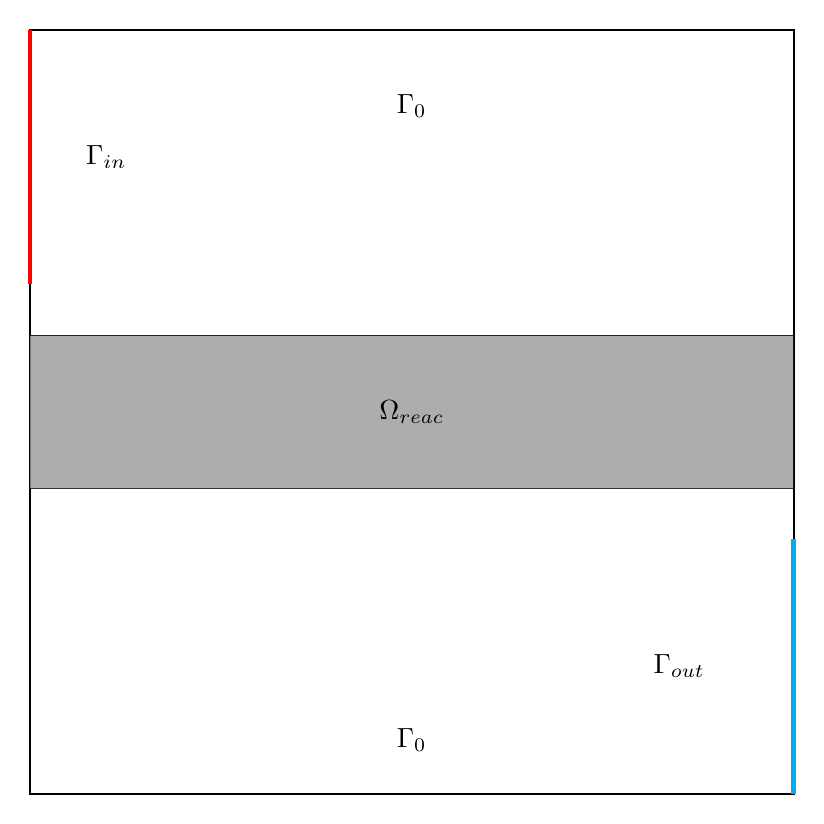
\begin{tikzpicture}[scale=0.8\textwidth/1cm]
      \draw[black,thick] (0.0,0.0) rectangle (1.0,1.0);
      %
      \draw[red,ultra thick] (0.0, 1.0) -- (0.0, 2./3);
      \node[black] at (0.1, 5/6) {$\Gamma_{in}$};
      %
      \draw[cyan,ultra thick] (1.0, 0.0) -- (1.0, 1./3);
      \node[black] at (0.85, 1/6) {$\Gamma_{out}$};
      %
      \node[black] at (0.5, 0.07) {$\Gamma_0$};
      \node[black] at (0.
      5, 0.9) {$\Gamma_0$};
      %
      \filldraw[fill=black!40!white, draw=black, opacity=0.8] (0.0, 0.4) rectangle (1.0, 0.6);
      \node[black] at (0.5,0.5) {$\Omega_{reac}$};
    \end{tikzpicture}
    \vspace*{0.5em}
    \caption{Problem setup}
  \end{subfigure}
  \hfill
  \begin{subfigure}{0.3\textwidth}
    \centering
    \includegraphics[width=0.9\textwidth]{figures/velocity_field.png}
    \caption{Velocity field $\vec{b}$}
  \end{subfigure}
  \hfill
  \begin{subfigure}{0.3\textwidth}
    \centering
    \includegraphics[width=0.9\textwidth]{figures/darcy_pressure.png}
    \caption{Pressure field $p$}
  \end{subfigure}\vspace*{-.2cm}
  \caption{\label{fig:testcases:catalysator} Problem setup and Darcy velocity field $\vec{b}$}\vspace*{-.5cm}
\end{figure}

The discretization scheme and the following experiments were implemented using the DUNE-framework~\cite{bastian2021dune} and the DUNE-PDELab discretization toolbox%
\footnote{\url{https://www.dune-project.org/modules/dune-pdelab}}.
%~\cite{dunepdelab}.
%\subsection{Problem formulation}
We consider the reactive transport of a pollutant inside a catalytic
filter. Let $\Omega$ be the unit square with boundary $\Gamma :=
\partial\Omega$. We assume that the velocity $\vec{b}$ is given
% by the Darcy-law, \ie
as the solution to the Darcy-equation
\begin{equation*}
%  \begin{cases}
    \nabla\cdot \vec{b} = 0, \qquad  
    \vec{b} = -k\nabla p \\
%  \end{cases}
\end{equation*}
subject to the boundary conditions
\begin{equation*}
  p = 1 \quad\text{on}\; \Gamma_{in}, \qquad
  p = 0 \quad\text{on}\; \Gamma_{out}, \qquad
  \vec{b} = 0 \quad\text{on}\; \Gamma_0 \;:= \Gamma \setminus (\Gamma_{in} \cup \Gamma_{out}).
\end{equation*}
Here, $k \in L^\infty(\Omega)$ denotes the permeability field. We introduce the reactive domain (washcoat) $\Omega_{reac} \subset \Omega$ and assume that the permeability in the reactive domain is significantly smaller, \ie $k = k_{min}\cdot\mathbbm{1}_{\Omega_{reac}} + \mathbbm{1}_{\Omega \backslash \Omega_{reac}}$, $k_{min}\in\R^+$. Similarly, the reaction function is given by $c = c_0 \cdot\mathbbm{1}_{\Omega_{reac}}$, $c_0\in\R^+$. All chosen parameters of the problem are summarized in Table~\ref{tab:params}.

\begin{table}[t]
  \begin{center}
    \renewcommand{\arraystretch}{1.4}
    \begin{tabular}{|c|c|c|c|c|c|c|c|}
    \hline
    $\Omega$ & $\Omega_{reac}$ & $\Gamma_{in}$ & $\Gamma_{out}$ & $g_D(z)$ & $f_\circ(x)$ & $k_{min}$ & $c_0$ \\
    \hline
    $[0,1]^2$ & $[0,1]\times [0.4,0.6]$ & $\{0\}\times (\tfrac{2}{3},1)$ & $\{1\} \times (0,\tfrac{1}{3})$ &$\sin(3\pi z)^2$ & $0$ & $10^{-1}$ & $0.5$ \\
    \hline
    \end{tabular}
  \end{center}
  \caption{Chosen parameters for the catalytic filter problem}\vspace*{-1cm}
  \label{tab:params}
\end{table}






%\subsection{Results}
In order to inspect the reconstruction $u^\delta$ we perform a voxel-wise evaluation on a refined mesh (\ie a projection into $\mathbb{P}^0$). In Fig.~\ref{fig:solutions} this is depicted alongside a solution obtained by a first order SIPG-method. In particular one notices nonaligned gradients when using a first order discretization of $\ycal$ (Fig.~\ref{fig:firstOrder}). However, since $u^\delta$ is only a $L^2$-like best approximation we do not expect $u^\delta$ to provide meaningful information \wrt the gradient (although the magnitude of the derivation still needs to converge in order to achieve $L^2$-convergence). Additionally, $u^\delta$ is the $\xcal_{L^2}$-best approximation from a non-standard space $\xcal^\delta$ where no information about its approximation qualities are given.

\begin{figure}[ht]
  \begin{subfigure}{0.315\textwidth}
    \centering
    \includegraphics[width=\linewidth]{figures/dg_solution.png}
    \caption{Solution computed with a first-order SIPG-scheme.}
  \end{subfigure}
  \hfill
  \begin{subfigure}{0.32\textwidth}
    \centering
    \includegraphics[width=.985\linewidth]{figures/ne_solution.png}
    \caption{\label{fig:firstOrder}Reconstructed solution for first order test functions.}
  \end{subfigure}
  \hfill
  \begin{subfigure}{0.345\textwidth}
    \centering
    \includegraphics[width=.92\linewidth]{figures/ne_solution_second_order.png}
    \caption{\label{fig:secondOrder}Reconstructed solution for second order test functions}
  \end{subfigure}\vspace*{-.2em}
%  \\
%  \hfill
%  \begin{subfigure}{0.25\textwidth}\label{fig:zoomFirstOrder}
%    \centering
%    \includegraphics[width=\linewidth]{figures/ne_solution_zoom.png}
%    %\caption{Zoom (first order)}
%  \end{subfigure}
%  \begin{subfigure}{0.25\textwidth}\label{fig:zoomSecondOrder}
%    \centering
%    \includegraphics[width=\linewidth]{figures/ne_solution_zoom_second_order.png}
%    %\caption{Zoom (second order)}
%  \end{subfigure}
  \caption{\label{fig:solutions} Solutions obtained by different discretization methods. All of them are based on a structued grid with $h^{-1}=40$.}\vspace*{-.5em}
\end{figure}


Finally, we investigate the convergence of the method under $h$-refinement. In~\cite{BrunkenSmetanaUrban}  the dependence of the convergence rate on the regularity of the inflow condition has already been established. Even for regular data only suboptimal rates have been observed with the optimal rate of $2$ for a linear FE space only attained in a one dimensional toy example. For the chosen catalytic filter problem we observe a convergence order of about $1.2$ for linear and $2.3$ for quadratic test functions (Fig.~\ref{fig:hconvergence}).

\begin{figure}[ht]
\centering
\begin{tikzpicture}
  \begin{loglogaxis}[
          width=0.5\linewidth, % Scale the plot to \linewidth
          grid=major, % Display a grid
          grid style={dashed,gray!30}, % Set the style
          xlabel=Global basis size, % Set the labels
          xlabel=grid width $h$,
          x dir=reverse,
          ylabel= $\norm{pr_{L^2}(u^\delta) - u_{SIPG}}_{L^2(\Omega)}$,
          legend style={at={(1.1,0.5)},anchor=west},
        ]

        \addplot[color=red , mark=x]
        table[x=gridwidth,y=l2error,col sep=comma] {conv_data_first_order.csv};
        \addlegendentry{first order};
        %
        \addplot[color=black, domain=5e-3:0.1]{10*x^(1.2)};
        \addlegendentry{$\mathcal{O}(h^{1.18})$};
        %
        \addplot[color=blue , mark=x]
        table[x=gridwidth,y=l2error,col sep=comma] {conv_data_second_order.csv};
        \addlegendentry{second order};
        %
        \addplot[color=black, dashed, domain=1e-2:0.1]{20*x^(2.3)};
        \addlegendentry{$\mathcal{O}(h^{2.28})$};
  \end{loglogaxis}
\end{tikzpicture}
\caption{\label{fig:hconvergence} Convergence under $h$-refinement}
\end{figure}
